%review for reading task 1 by Zhe Yan%
\documentclass{article}
\usepackage[top=1in, bottom=1in, left=1.25in, right=1.25in]{geometry}
\usepackage{amsmath}
\usepackage{graphicx}
\graphicspath{ {C:/Users/JJ/Desktop/} }
\usepackage[export]{adjustbox}
\usepackage{subcaption}
\usepackage{fancyhdr}\pagestyle{fancy}
%\usepackage{algorithmic}
\usepackage[]{algorithm2e}
\usepackage{bm}
\begin{document}
\newcommand{\lfront}{\fontsize{17.28pt}{\baselineskip}\selectfont}
\newcommand{\mfront}{\fontsize{12pt}{\baselineskip}\selectfont}
\newcommand{\sfront}{\fontsize{9pt}{\baselineskip}\selectfont}
\fancyhead[L]{\sfront{Jiejie Wei	\&	Bumsik Kim}}
\fancyhead[R]{\sfront{\today}}
\begin{center}
\lfront{\textbf{Robot Simulation}}
\end{center}

\section{Summary}
\qquad Our project is to develop algorithms and protocols for the localization of sensors and mobile robots. We focus more on the analysis and modelling using simulation tools.  \\

	


\section{Simulation Program}
\qquad Our first task is to simulate random location of robots in Matlab. Each robot should have three ranges, sensory range, communication range and reject range. Sensory range is the largest range that allows each of robots to sense each other within that area. Communication range is the smaller range that allows robots to communicate with each other. Reject range is the smallest range in the case when two robots are too close, they can't sense each other, which is what we want to avoid during the simulation. In order to do this, we create three files, described as following:
\begin{itemize}
\item "drawCircle.m": A simple function to draw circle with parameters x,y and r which stands for the locations and radius. \item "Robot.m": A class that has properties called "sensory", "communication" and "reject" which hold values for the radius of each range. Properties "x" and "y" stands for the location of robots in graph to be drawn. This class has four methods of drawing circles, "drawSensory(obj)", "drawCommunication(obj)", "drawReject(obj)" and "drawAll(obj)" which can draw three types of circle range individually and in one time. 
\item "simulation.m": The driver file that creates 8 robot object in random location in the graph. In order to avoid robots correlated with each other within the reject range, the algorithm is to keep looking for the position of a new robot until the condition satisfied and then create robot according to that position. 
\end{itemize}

\section{Simulation Result}
\indent The following graphs are 4 simulation results that randomly allocate 8 robot objects:\\
 
\begin{figure}[h]
 
\begin{subfigure}{0.24\textwidth}
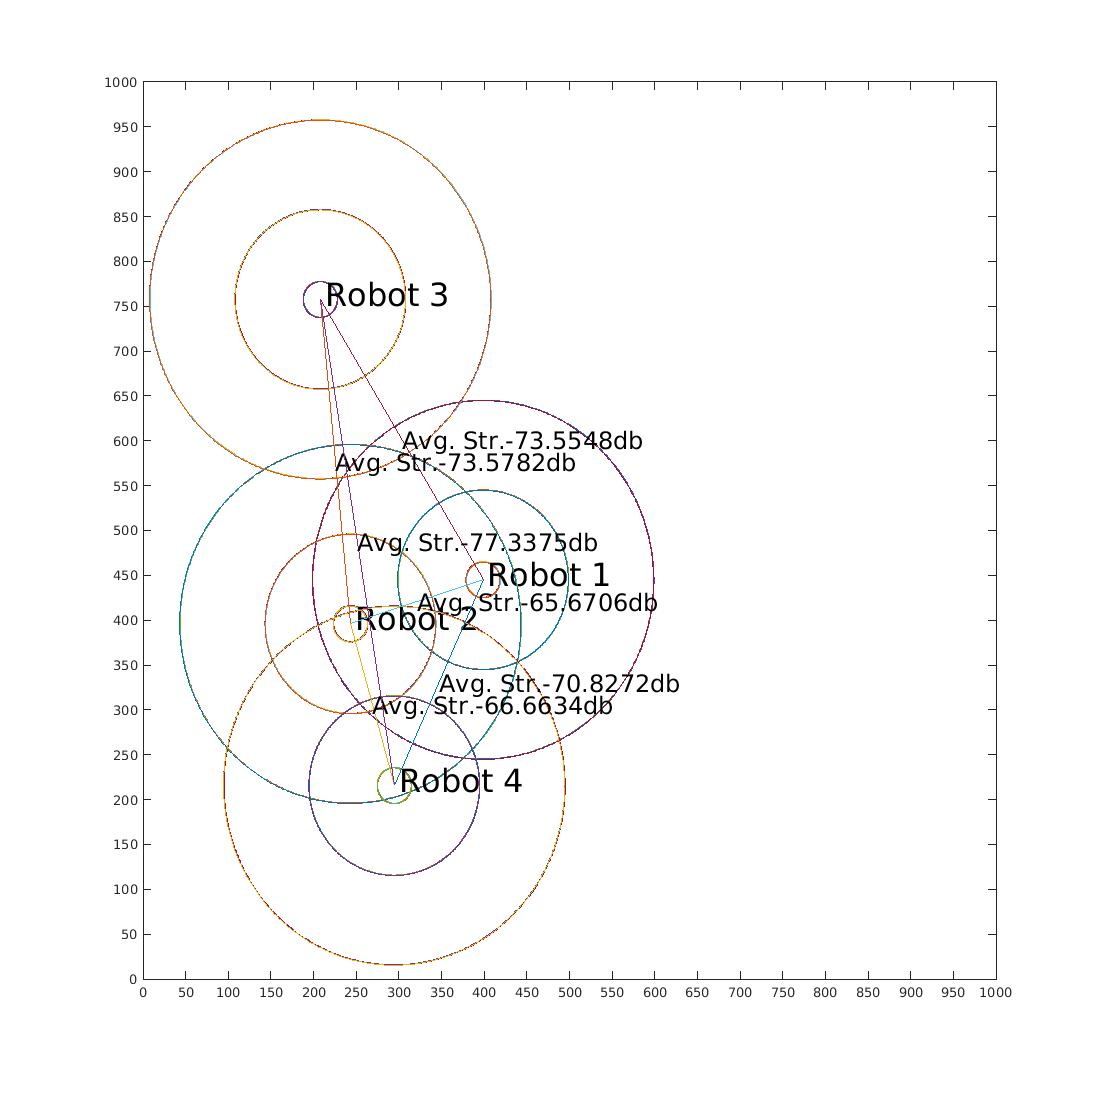
\includegraphics[width=0.9\linewidth]{simulation1} 
\caption{Sample simulation 1}
\label{fig:subim1}
\end{subfigure}
\begin{subfigure}{0.24\textwidth}
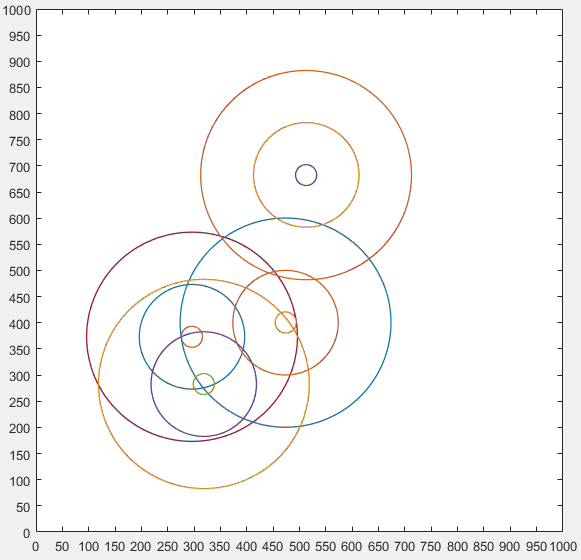
\includegraphics[width=0.9\linewidth]{simulation2}
\caption{Sample simulation 2}
\label{fig:subim2}
\end{subfigure}
\begin{subfigure}{0.24\textwidth}
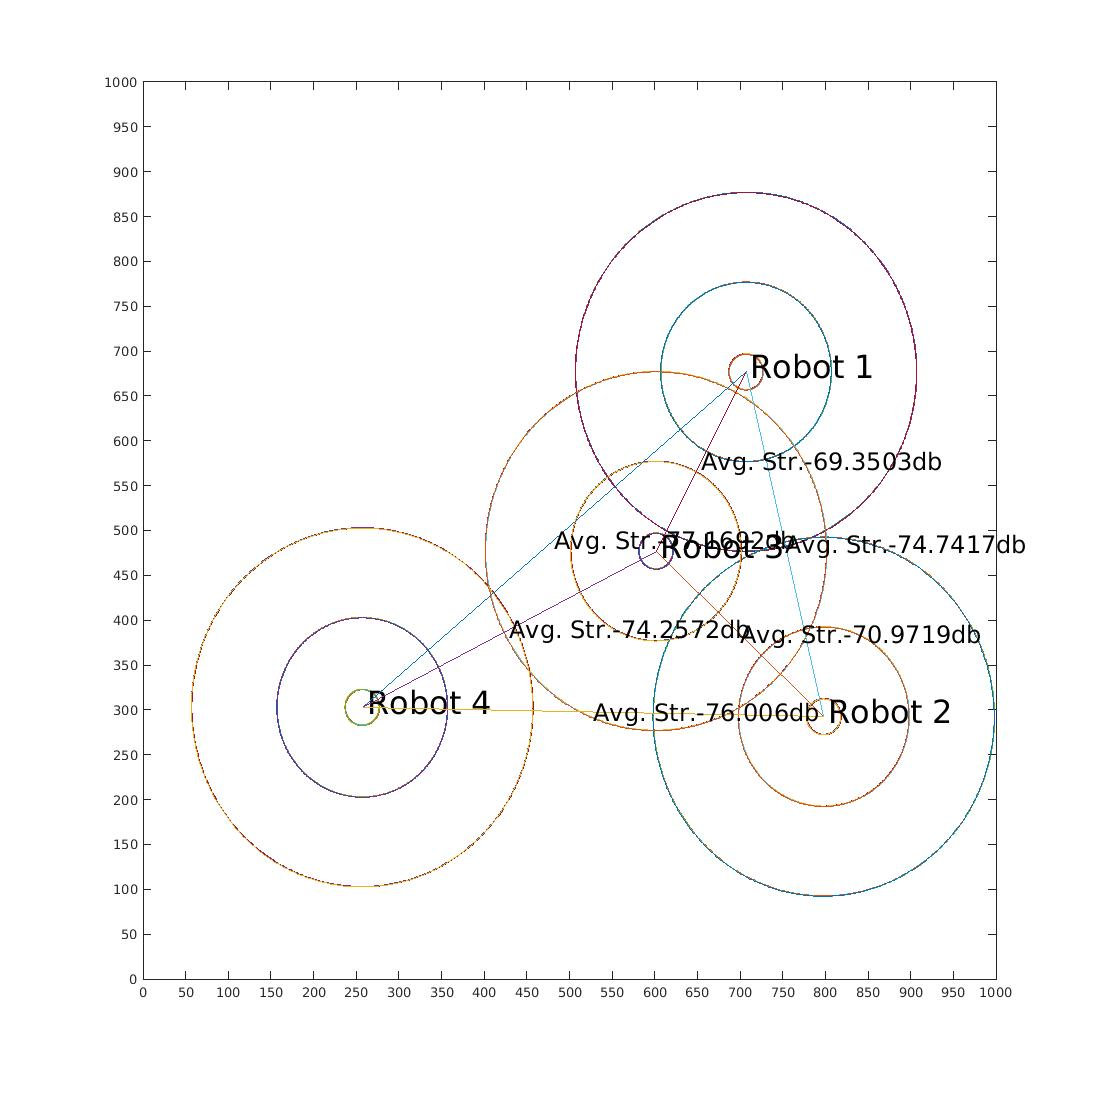
\includegraphics[width=0.9\linewidth]{simulation3}
\caption{Sample simulation 3}
\label{fig:subim3}
\end{subfigure}
\begin{subfigure}{0.24\textwidth}
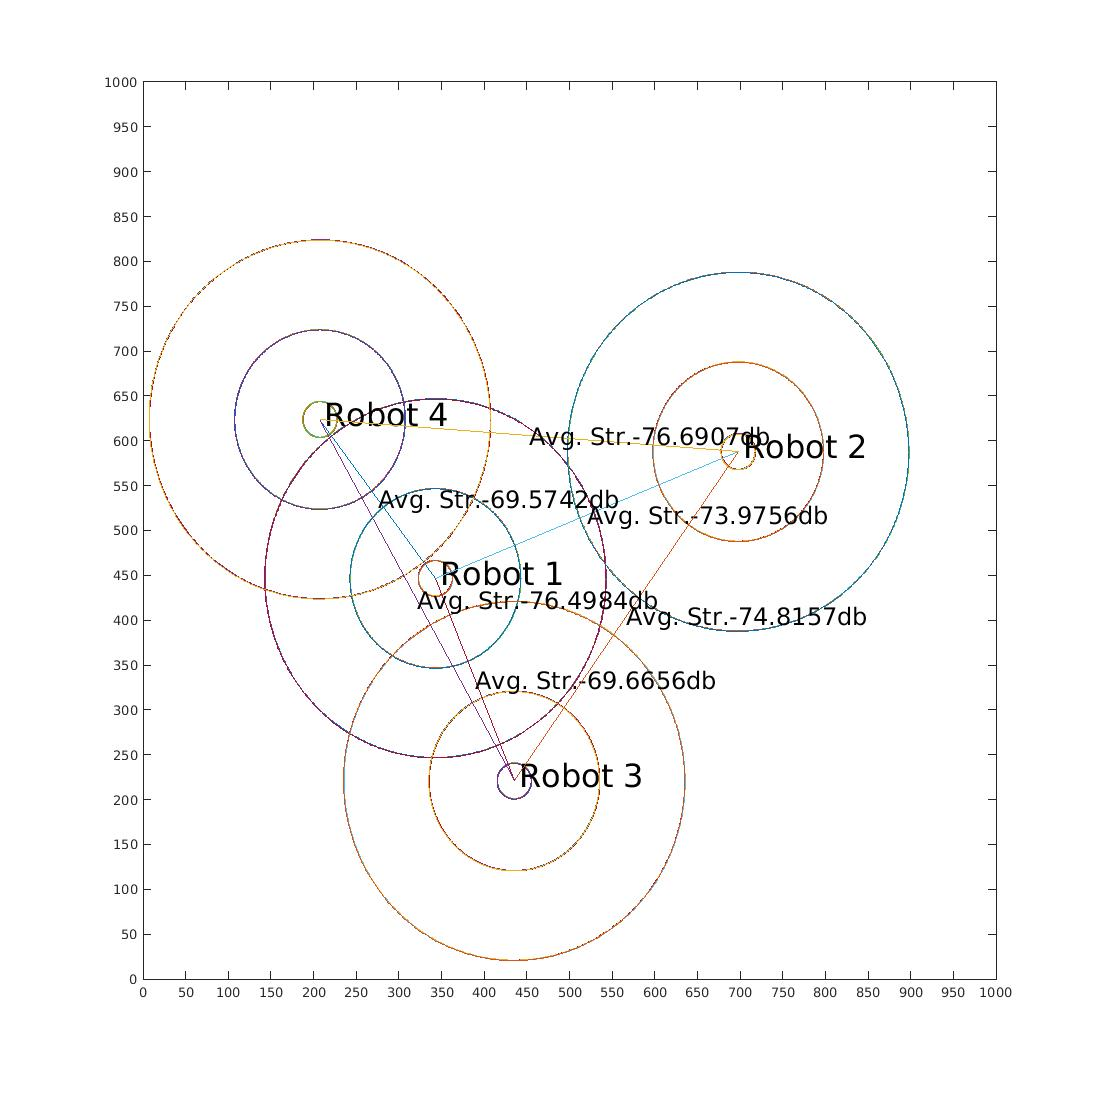
\includegraphics[width=0.9\linewidth]{simulation4}
\caption{Sample simulation 4}
\label{fig:subim4}
\end{subfigure}

\caption{Four sample simulations}
\label{fig:image2}
\end{figure}



\end{document}
